\section{YAZILIM GELİŞTİRME}

\subsection{Yaya Geçidi Otomatik Tespit Algoritması}

Sistem açıldığında önce \texttt{crosswalk.json} dosyasına kayıtlı bölge koordinatları kontrol edilir. Geçerli bir kayıt bulunamazsa \texttt{crosswalk\_detector.py} içindeki otomatik tespit rutini çalıştırılır. Algoritma aşağıdaki adımlardan oluşmaktadır:

\begin{enumerate}
  \item \textbf{Ön İşleme:} Gri tonlamalı görüntüye CLAHE (Kontrast Sınırlı Adaptif Histogram Eşitleme) uygulanır. Ardından Gauss bulanıklaştırması ($5\times5$ çekirdek) ile gürültü azaltılır.
  \item \textbf{Kenar Tespiti:} Canny algoritması $[30, 90]$ eşik değerleriyle çalıştırılır:
    \begin{equation}
      G = \sqrt{G_x^2 + G_y^2}, \quad \theta = \arctan\!\left(\frac{G_y}{G_x}\right)
    \end{equation}
  \item \textbf{Hough Dönüşümü:} \texttt{HoughLinesP} fonksiyonu uygulanır (eşik: 50, minLineLength: 50, maxLineGap: 10). Çıktı çizgilerden yalnızca yatay olanlar ($|\theta| \leq 15°$) seçilir; bu çizgiler yaya geçidi yatay şerit adayları olarak kabul edilir.
  \item \textbf{Gap-Clustering:} $y$ ekseninde birbirine 18 pikselden yakın çizgiler aynı kümeye atanır. Her küme bir yaya geçidi şeridini temsil eder.
  \item \textbf{Tutarlılık Kontrolü:} Geçerli bir yaya geçidi için şu koşulların tamamı sağlanmalıdır:
    \begin{itemize}
      \item Küme sayısı $\geq 3$
      \item Küme $y$-koordinatları varyasyon katsayısı $\leq 0.65$
      \item Tespit edilen bölge genişliği $\geq$ görüntü genişliğinin \%15'i
    \end{itemize}
  \item \textbf{Sonuç:} Başarılı tespit durumunda bölge sınırlayıcı kutusundan dört köşe noktası hesaplanır ve \texttt{crosswalk.json}'a kaydedilir. Başarısız olunması durumunda \texttt{crosswalk\_setup.py} interaktif seçici başlatılır.
\end{enumerate}

\begin{figure}[H]
\centering
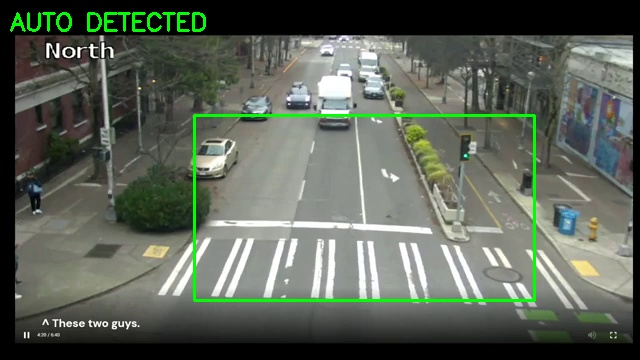
\includegraphics[width=0.75\textwidth]{debug_detection.jpg}
\caption{Canny+HoughLinesP ile otomatik yaya geçidi tespit sonucu}
\label{fig:tespit}
\end{figure}

\subsection{Durum Makinesi}

Çalışma sırasında sistem, her işlenen kare için üç durumdan birinde bulunur. Durum geçişleri Tablo~\ref{tbl:durumlar}'de özetlenmiştir.

\begin{table}[H]
\centering
\caption{SmartWalk Durum Makinesi}
\label{tbl:durumlar}
\begin{tabular}{|l|p{5cm}|p{5cm}|}
\hline
\textbf{Durum}             & \textbf{Koşul}                          & \textbf{Eylem} \\
\hline
\texttt{GÜVENLI}           & Bölgede araç veya yaya yok              & Pasif izleme, ekranda yeşil gösterge \\
\hline
\texttt{YAYA ALGILANDI}    & Bölgede yalnızca yaya var               & Uyarı rengi (sarı), araç bekleme \\
\hline
\texttt{İHLAL}             & Bölgede hem araç hem de yaya var (N$\geq$2 kare onay) & Fotoğraf kaydet, Telegram bildir, Firebase logla, 30~s cooldown \\
\hline
\end{tabular}
\end{table}

İhlal kararı vermek için N ardışık kare onayı (\texttt{VIOLATION\_CONFIRM} parametresi, varsayılan: 2) aranır; bu yöntem anlık algılama hatalarından kaynaklanan yanlış pozitifleri azaltır.

\subsection{İhlal Yönetimi ve Thread Mimarisi}

\texttt{violation\_handler.py} içindeki \texttt{ViolationHandler} sınıfı, ihlal bildirimlerini ana görüntü işleme döngüsünden bağımsız bir \texttt{threading.Thread} içinde yönetir. İhlal tespiti yapıldığında ana döngü yalnızca bir kare kopyasını ve meta veriyi kuyruğa (\texttt{queue.Queue}) ekler; arka plan thread'i bu kuyruğu tüketerek fotoğrafı diske kaydeder, Telegram mesajını gönderir ve Firebase kaydını oluşturur. Bu mimari sayesinde ağ gecikmesi veya disk yazma süresinden bağımsız olarak ana döngü çalışmaya devam eder.

Cooldown mekanizması, son ihlal zamanı ile mevcut zaman arasındaki fark 30 saniyeden (\texttt{COOLDOWN\_SECONDS}) küçükse yeni bildirimi engelleyerek aynı ihlal için tekrarlı mesaj gönderimini önler.

\subsection{ESP32 MJPEG Stream Okuyucu}

\texttt{esp32\_stream.py} içindeki \texttt{ESP32MJPEGCapture} sınıfı, HTTP yanıtının byte akışını okuyarak JPEG çerçevelerini JPEG SOI (\texttt{0xFF 0xD8}) ve EOI (\texttt{0xFF 0xD9}) marker'larına göre ayıklar. OpenCV'nin \texttt{VideoCapture} sınıfı MJPEG boundary bazlı ayrıştırmada tutarsız davranabildiğinden, bu düşük seviye yaklaşım tercih edilmiştir.

\begin{lstlisting}[caption={ESP32MJPEGCapture -- JPEG marker tabanlı çerçeve ayıklama}, label={lst:mjpeg}]
class ESP32MJPEGCapture:
    def __init__(self, url: str, timeout: int = 10):
        self.url = url
        self.timeout = timeout
        self._stream = None
        self._buffer = b""

    def connect(self) -> bool:
        try:
            resp = requests.get(self.url, stream=True,
                                timeout=self.timeout)
            self._stream = resp.iter_content(chunk_size=4096)
            return True
        except Exception as e:
            print(f"Baglanti hatasi: {e}")
            return False

    def read_frame(self):
        while True:
            chunk = next(self._stream, None)
            if chunk is None:
                return False, None
            self._buffer += chunk
            soi = self._buffer.find(b"\xff\xd8")
            eoi = self._buffer.find(b"\xff\xd9", soi)
            if soi != -1 and eoi != -1:
                jpg = self._buffer[soi:eoi + 2]
                self._buffer = self._buffer[eoi + 2:]
                frame = cv2.imdecode(
                    np.frombuffer(jpg, dtype=np.uint8),
                    cv2.IMREAD_COLOR
                )
                return frame is not None, frame
\end{lstlisting}

\begin{lstlisting}[caption={SmartWalkDetector -- YOLOv8n çıkarımı ve sınıf filtresi}, label={lst:detector}]
DETECT_CLASSES = {0: "kisi", 2: "arac",
                  3: "motorsiklet", 5: "otobus", 7: "kamyon"}

class SmartWalkDetector:
    def __init__(self, model_path: str = "yolov8n.pt",
                 conf: float = 0.40):
        self.model = YOLO(model_path)
        self.conf = conf

    def detect(self, frame):
        results = self.model(frame, conf=self.conf,
                             verbose=False)[0]
        detections = sv.Detections.from_ultralytics(results)
        mask = np.isin(detections.class_id,
                       list(DETECT_CLASSES.keys()))
        return detections[mask]
\end{lstlisting}

\begin{lstlisting}[caption={CrosswalkZone -- polygon içi tespit filtresi}, label={lst:zone}]
class CrosswalkZone:
    def __init__(self, polygon: np.ndarray):
        # polygon: (4,2) array, saat yonunde koseler
        self.polygon = polygon

    def contains(self, detections: sv.Detections) -> sv.Detections:
        if len(detections) == 0:
            return detections
        cx = (detections.xyxy[:, 0] +
              detections.xyxy[:, 2]) / 2
        cy = (detections.xyxy[:, 1] +
              detections.xyxy[:, 3]) / 2
        pts = np.stack([cx, cy], axis=1).astype(np.float32)
        inside = np.array([
            cv2.pointPolygonTest(
                self.polygon.astype(np.float32), tuple(p), False
            ) >= 0
            for p in pts
        ])
        return detections[inside]
\end{lstlisting}

\begin{lstlisting}[caption={main.py -- Ana durum makinesi döngüsü (özet)}, label={lst:main}]
def run_loop(cap, detector, zone, handler, args):
    frame_idx = 0
    violation_counter = 0
    for raw_ok, frame in cap:
        if not raw_ok:
            break
        frame_idx += 1
        if frame_idx % args.frame_skip != 0:
            continue
        dets = detector.detect(frame)
        in_zone = zone.contains(dets)
        has_person  = any(d == 0 for d in in_zone.class_id)
        has_vehicle = any(d in {2,3,5,7}
                          for d in in_zone.class_id)
        if has_person and has_vehicle:
            violation_counter += 1
        else:
            violation_counter = 0
        if violation_counter >= args.confirm:
            handler.report(frame, in_zone)
            violation_counter = 0
\end{lstlisting}

